\section{PROJECT MANAGEMENT}
\subsection{Updated Schedule}
    \begin{figure}[thpb]
        \parbox{\linewidth}{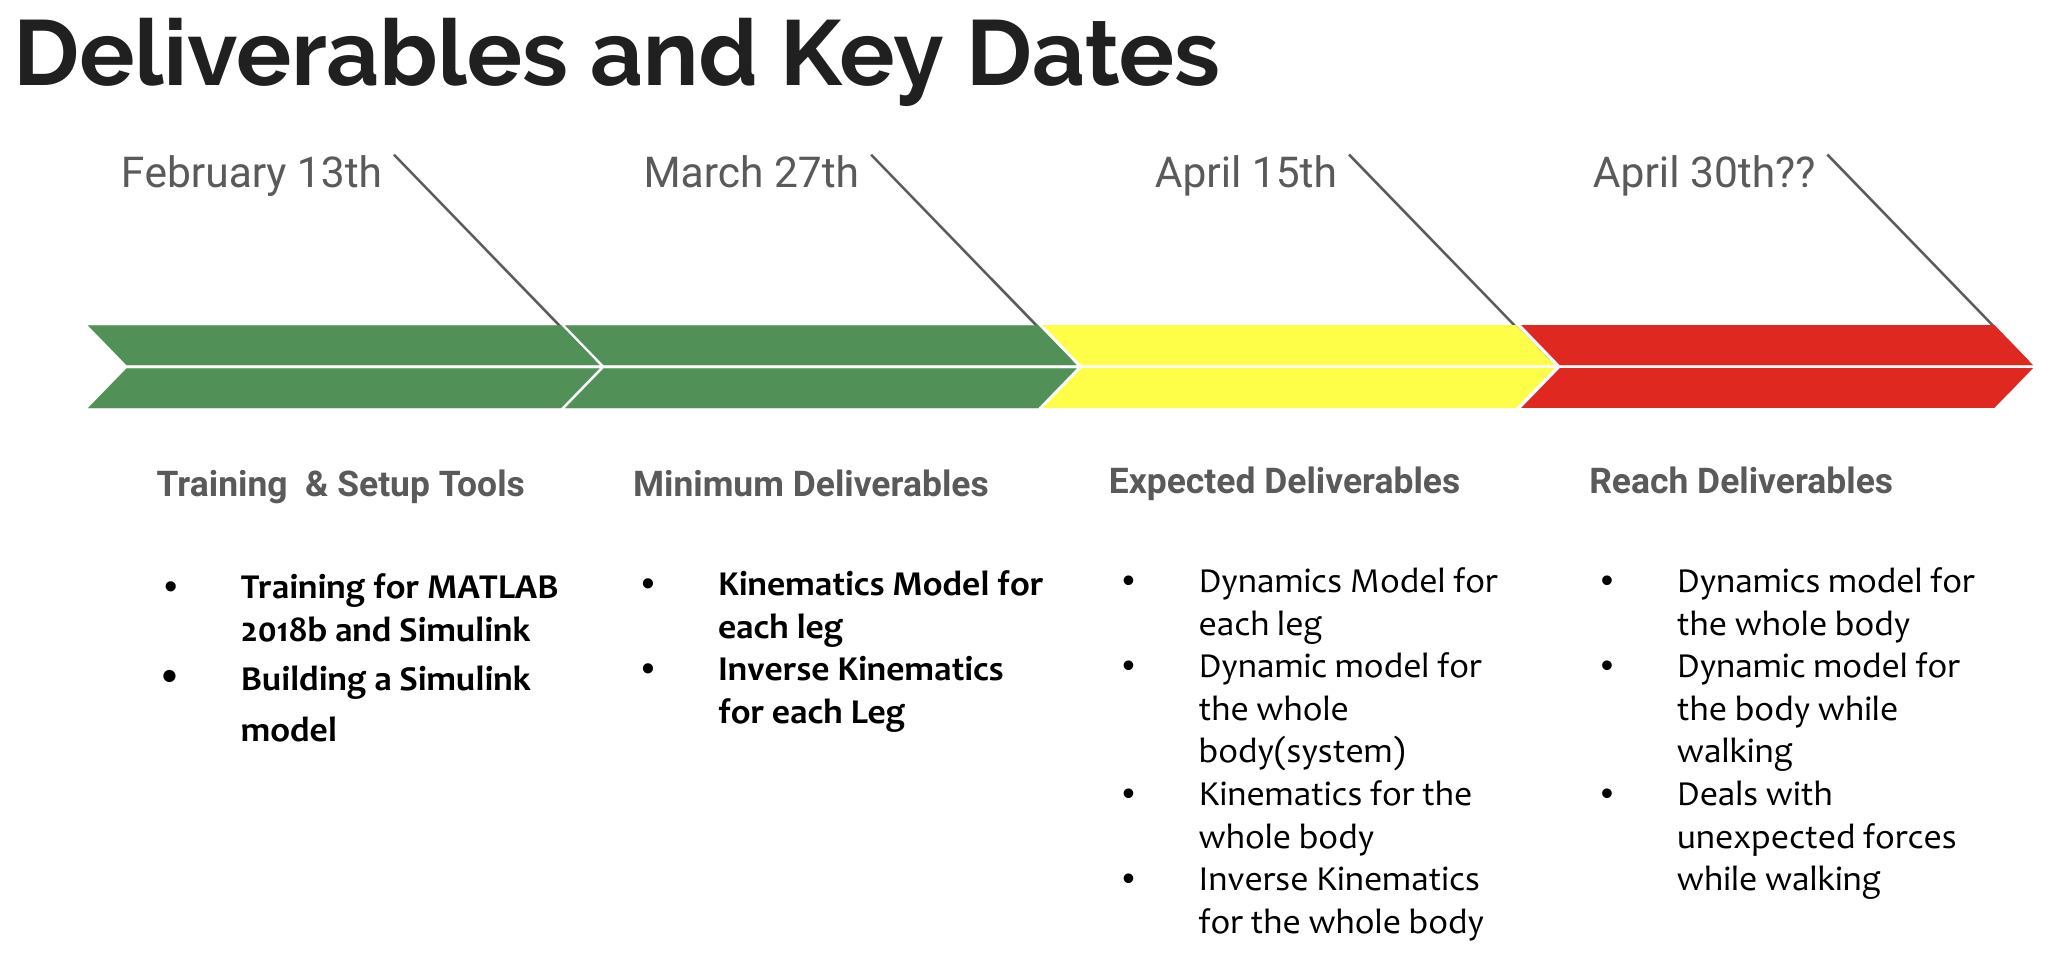
\includegraphics[width=\linewidth]{Figures/UpdatedSchedule.png}}
        \caption{Our updated schedule. Bolded tasks have been completed}
        \label{fig:updatedschedule}
    \end{figure}
\subsection{Dependencies}
We have two major dependencies coming into the second half of our project: our dynamic model for our leg and our dynamic model for our body. As seen in the schedule, we want to not only model our quadruped, but also give it basic control over its body. This will require a bullet proof model for each leg, which will be used for a dynamic body model. Although this is our reach goal, we hope to finish it within the next few weeks, and to have a demo ready.
\subsection{Challenges}
Like any project, we ran into a few major issues that slowed our progress more than expected. The first of these problems were our 4 DoF leg. Unlike most quadrupeds, our leg design has a single roll joint, with a planar 3DoF manipulator. This configuration allows us to have nearly unlimited attack angles to the ground, but also introduces a lot of complexity when calculating inverse kinematics and modeling the dynamics of the leg.

We also ran into problems when dynamically modeling the legs themselves. No group member had experience in dynamic modeling, so we studied literature and asked professors to learn how dynamic modeling worked in a case like ours. We also simplified the model (see Section \ref{sec:CAD Model Design}), to make the modeling process easier.

Our final major problem we faced was our inexperience with MATLAB SimMechanics modeling. This inexperience led to many refactors of our code base, and although another refactor may happen in the near future, we think that our software is at a point where we can continue development with less distractions.